\documentclass[10pt]{article}
\usepackage[paperwidth=11in,paperheight=8.5in,margin=.45in,footskip=16pt]{geometry}
\usepackage[T1]{fontenc}\usepackage{lmodern}\usepackage{booktabs,longtable,array,pgfplots}
\pgfplotsset{compat=1.18}\setlength{\parindent}{0pt}
\begin{document}
{\LARGE\bfseries Baseline welfare: completed primary profiles}\par\medskip
Coverage: 72 of 74 article-selected primary cases; 34 of 36 American/British comparisons. Pending cases are listed in the source data.\par\smallskip
These are five separate monetary measures, in damages units and weighted over potential disputes. They do not form an additive welfare index. The truth relationship is the baseline identity map. Alternative truth assumptions are not included.\par\smallskip
RN denotes risk neutrality; RA denotes symmetric CARA risk aversion (alpha in parentheses). Asymmetric cases state each party\textquotesingle s alpha. American and British are the main rules. Trial-only fee shifting appears as a separate ordinary-cost extension.\par\smallskip
Levels use the established truth-prior weighting of truth-conditional outcomes; direct replay truth mass is retained separately in the source catalog. Values are displayed to three decimals; calculations and comparisons use unrounded data. $\dagger$ marks a nonzero value that rounds to zero.\par\medskip
\small\setlength{\tabcolsep}{4pt}
\begin{longtable}{@{}p{3.0in}llrrrrr@{}}
\toprule Specification & Risk & Fee & P shortfall & D nonliable & D liable excess & Gross error & Real costs\\\midrule\endfirsthead
\toprule Specification & Risk & Fee & P shortfall & D nonliable & D liable excess & Gross error & Real costs\\\midrule\endhead
\bottomrule\endfoot
Baseline; cost 0.25 & RA (2) & American & 0.201 & 0.197 & 0.004 & 0.354 & 0.088\\
Baseline; cost 0.25 & RA (2) & British & 0.190 & 0.187 & 0.005 & 0.338 & 0.086\\
Baseline; cost 0.25 & RN & American & 0.182 & 0.182 & 0.022 & 0.294 & 0.138\\
Baseline; cost 0.25 & RN & British & 0.167 & 0.155 & 0.045 & 0.285 & 0.114\\
Baseline; cost 0.5 & RA (2) & American & 0.223 & 0.219 & 0.008 & 0.354 & 0.175\\
Baseline; cost 0.5 & RA (2) & British & 0.200 & 0.231 & 0.005 & 0.352 & 0.161\\
Baseline; cost 0.5 & RN & American & 0.201 & 0.189 & 0.032 & 0.282 & 0.207\\
Baseline; cost 0.5 & RN & British & 0.178 & 0.160 & 0.072 & 0.280 & 0.176\\
Baseline; cost 1 & RA (2) & American & 0.278 & 0.278 & 0.004 & 0.399 & 0.312\\
Baseline; cost 1 & RA (2) & British & 0.168 & 0.156 & 0.064 & 0.277 & 0.142\\
Baseline; cost 1 & RA (2) & Trial only & 0.196 & 0.184 & 0.014 & 0.280 & 0.175\\
Baseline; cost 1 & RN & American & 0.216 & 0.222 & 0.028 & 0.278 & 0.292\\
Baseline; cost 1 & RN & British & 0.167 & 0.197 & 0.096 & 0.275 & 0.262\\
Baseline; cost 1 & RN & Trial only & 0.213 & 0.175 & 0.047 & 0.273 & 0.236\\
Baseline; cost 2 & RA (2) & American & 0.277 & 0.163 & 0.006 & 0.281 & 0.256\\
Baseline; cost 2 & RA (2) & British & 0.169 & 0.204 & 0.113 & 0.285 & 0.258\\
Baseline; cost 2 & RN & American & 0.274 & 0.220 & 0.023 & 0.282 & 0.361\\
Baseline; cost 2 & RN & British & 0.183 & 0.199 & 0.142 & 0.275 & 0.321\\
Baseline; cost 4 & RA (2) & American & 0.426 & 0.058 & 0.001 & 0.341 & 0.190\\
Baseline; cost 4 & RA (2) & British & 0.237 & 0.205 & 0.187 & 0.297 & 0.413\\
Baseline; cost 4 & RN & American & 0.343 & 0.346 & 0.007 & 0.328 & 0.607\\
Baseline; cost 4 & RN & British & 0.215 & 0.198 & 0.230 & 0.283 & 0.421\\
asymmetric-risk / d-only-ra; cost 1 & P 0, D 2 & American & 0.210 & 0.268 & 0.024 & 0.304 & 0.318\\
asymmetric-risk / d-only-ra; cost 1 & P 0, D 2 & British & 0.106 & 0.313 & 0.076 & 0.314 & 0.261\\
asymmetric-risk / p-only-ra; cost 1 & P 2, D 0 & American & 0.268 & 0.166 & 0.024 & 0.304 & 0.259\\
asymmetric-risk / p-only-ra; cost 1 & P 2, D 0 & British & 0.292 & 0.103 & 0.021 & 0.320 & 0.165\\
cost-timing / earlier-costs; cost 1 & RA (2) & American & 0.272 & 0.270 & 0.018 & 0.333 & 0.391\\
cost-timing / earlier-costs; cost 1 & RA (2) & British & 0.294 & 0.229 & 0.028 & 0.338 & 0.376\\
cost-timing / earlier-costs; cost 1 & RN & American & 0.238 & 0.204 & 0.026 & 0.275 & 0.290\\
cost-timing / earlier-costs; cost 1 & RN & British & 0.177 & 0.175 & 0.109 & 0.275 & 0.235\\
cost-timing / later-costs; cost 1 & RA (2) & American & 0.242 & 0.242 & 0.004 & 0.399 & 0.168\\
cost-timing / later-costs; cost 1 & RA (2) & British & 0.165 & 0.157 & 0.041 & 0.283 & 0.113\\
cost-timing / later-costs; cost 1 & RN & American & 0.226 & 0.203 & 0.042 & 0.280 & 0.288\\
cost-timing / later-costs; cost 1 & RN & British & 0.170 & 0.172 & 0.069 & 0.273 & 0.195\\
court-noise / sigma-0p1; cost 1 & RA (2) & American & 0.254 & 0.254 & 0.011 & 0.340 & 0.336\\
court-noise / sigma-0p1; cost 1 & RA (2) & British & 0.167 & 0.155 & 0.064 & 0.276 & 0.142\\
court-noise / sigma-0p1; cost 1 & RN & American & 0.214 & 0.203 & 0.025 & 0.269 & 0.266\\
court-noise / sigma-0p1; cost 1 & RN & British & 0.164 & 0.165 & 0.085 & 0.268 & 0.195\\
court-noise / sigma-0p4; cost 1 & RA (2) & American & 0.317 & 0.317 & 0.001 & 0.483 & 0.303\\
court-noise / sigma-0p4; cost 1 & RA (2) & British & 0.319 & 0.319 & 0.001 & 0.487 & 0.301\\
court-noise / sigma-0p4; cost 1 & RN & American & 0.329 & 0.329 & 0.075 & 0.383 & 0.552\\
court-noise / sigma-0p4; cost 1 & RN & British & 0.281 & 0.211 & 0.120 & 0.328 & 0.377\\
direct-binary / calibrated-to-uniform-merits; cost 1 & RA (2) & American & 0.281 & 0.281 & 0.004 & 0.407 & 0.309\\
direct-binary / calibrated-to-uniform-merits; cost 1 & RA (2) & British & 0.200 & 0.200 & 0.012 & 0.256 & 0.309\\
direct-binary / calibrated-to-uniform-merits; cost 1 & RN & American & 0.140 & 0.102 & 0.047 & 0.080 & 0.283\\
direct-binary / calibrated-to-uniform-merits; cost 1 & RN & British & 0.054 & 0.043 & 0.117 & 0.076 & 0.222\\
grid / signals-12-offers-8; cost 1 & RA (2) & American & 0.262 & 0.262 & 0.011 & 0.356 & 0.336\\
grid / signals-12-offers-8; cost 1 & RN & American & 0.228 & 0.198 & 0.033 & 0.276 & 0.274\\
grid / signals-12-offers-8; cost 1 & RN & British & 0.166 & 0.189 & 0.091 & 0.274 & 0.236\\
grid / signals-8-offers-15; cost 1 & RA (2) & American & 0.290 & 0.290 & 0.003 & 0.425 & 0.309\\
grid / signals-8-offers-15; cost 1 & RN & American & 0.233 & 0.233 & 0.031 & 0.293 & 0.324\\
grid / signals-8-offers-15; cost 1 & RN & British & 0.179 & 0.175 & 0.095 & 0.275 & 0.230\\
grid / signals-8-offers-8; cost 1 & RA (2) & American & 0.290 & 0.290 & 0.003 & 0.425 & 0.309\\
grid / signals-8-offers-8; cost 1 & RA (2) & British & 0.264 & 0.146 & 0.007 & 0.317 & 0.200\\
grid / signals-8-offers-8; cost 1 & RN & American & 0.220 & 0.222 & 0.031 & 0.277 & 0.303\\
grid / signals-8-offers-8; cost 1 & RN & British & 0.179 & 0.175 & 0.095 & 0.275 & 0.230\\
merits-distribution / center-weighted; cost 1 & RA (2) & American & 0.290 & 0.319 & 0.006 & 0.450 & 0.317\\
merits-distribution / center-weighted; cost 1 & RA (2) & British & 0.311 & 0.309 & 0.002 & 0.468 & 0.303\\
merits-distribution / center-weighted; cost 1 & RN & American & 0.303 & 0.303 & 0.047 & 0.376 & 0.457\\
merits-distribution / center-weighted; cost 1 & RN & British & 0.239 & 0.242 & 0.119 & 0.346 & 0.350\\
merits-distribution / polarized; cost 1 & RA (2) & American & 0.227 & 0.227 & 0.008 & 0.291 & 0.326\\
merits-distribution / polarized; cost 1 & RA (2) & British & 0.119 & 0.114 & 0.067 & 0.202 & 0.120\\
merits-distribution / polarized; cost 1 & RN & American & 0.181 & 0.139 & 0.019 & 0.200 & 0.200\\
merits-distribution / polarized; cost 1 & RN & British & 0.127 & 0.122 & 0.087 & 0.200 & 0.174\\
private-noise / sigma-0p1; cost 1 & RA (2) & American & 0.247 & 0.243 & 0.003 & 0.335 & 0.310\\
private-noise / sigma-0p1; cost 1 & RA (2) & British & 0.159 & 0.127 & 0.057 & 0.259 & 0.093\\
private-noise / sigma-0p1; cost 1 & RN & American & 0.209 & 0.160 & 0.017 & 0.261 & 0.182\\
private-noise / sigma-0p1; cost 1 & RN & British & 0.160 & 0.170 & 0.080 & 0.261 & 0.182\\
private-noise / sigma-0p4; cost 1 & RA (2) & American & 0.300 & 0.350 & 0.000 & 0.500 & 0.300\\
private-noise / sigma-0p4; cost 1 & RA (2) & British & 0.350 & 0.300 & 0.000 & 0.500 & 0.300\\
private-noise / sigma-0p4; cost 1 & RN & American & 0.292 & 0.292 & 0.089 & 0.308 & 0.553\\
private-noise / sigma-0p4; cost 1 & RN & British & 0.241 & 0.214 & 0.151 & 0.310 & 0.450\\
\end{longtable}\normalsize
\newpage
{\LARGE\bfseries Matched fee comparisons}\par\medskip
Every difference is British minus American under the same specification, costs and risk preferences. Signed magnitudes are shown without combining unlike cases or interpreting their frequency as a probability. Each listed pair has passed the four-corner rule/behavior decomposition and complete endpoint checks.\par\medskip
\small\begin{longtable}{@{}lp{3.0in}lrrrrr@{}}
\toprule Code & Specification & Risk & P shortfall & D nonliable & D liable excess & Gross error & Real costs\\\midrule\endfirsthead
\toprule Code & Specification & Risk & P shortfall & D nonliable & D liable excess & Gross error & Real costs\\\midrule\endhead
\bottomrule\endfoot
C01 & asymmetric-risk / d-only-ra; cost 1 & P 0, D 2 & -0.104 & 0.045 & 0.053 & 0.010 & -0.057\\
C02 & asymmetric-risk / p-only-ra; cost 1 & P 2, D 0 & 0.024 & -0.063 & -0.003 & 0.015 & -0.095\\
C03 & Baseline; cost 1 & RA (2) & -0.110 & -0.122 & 0.060 & -0.122 & -0.170\\
C04 & Baseline; cost 1 & RN & -0.049 & -0.025 & 0.068 & -0.002 & -0.030\\
C05 & Baseline; cost 0.25 & RA (2) & -0.011 & -0.010 & 0.001 & -0.016 & -0.002\\
C06 & Baseline; cost 0.5 & RA (2) & -0.023 & 0.012 & -0.002 & -0.001 & -0.014\\
C07 & Baseline; cost 2 & RA (2) & -0.107 & 0.041 & 0.106 & 0.005 & 0.002\\
C08 & Baseline; cost 4 & RA (2) & -0.189 & 0.147 & 0.186 & -0.044 & 0.223\\
C09 & Baseline; cost 0.25 & RN & -0.015 & -0.026 & 0.023 & -0.009 & -0.024\\
C10 & Baseline; cost 0.5 & RN & -0.023 & -0.029 & 0.040 & -0.003 & -0.031\\
C11 & Baseline; cost 2 & RN & -0.091 & -0.021 & 0.120 & -0.007 & -0.041\\
C12 & Baseline; cost 4 & RN & -0.128 & -0.148 & 0.223 & -0.046 & -0.185\\
C13 & cost-timing / earlier-costs; cost 1 & RA (2) & 0.023 & -0.041 & 0.010 & 0.005 & -0.015\\
C14 & cost-timing / earlier-costs; cost 1 & RN & -0.061 & -0.029 & 0.083 & 0.000$^{\dagger}$ & -0.055\\
C15 & cost-timing / later-costs; cost 1 & RA (2) & -0.077 & -0.084 & 0.037 & -0.116 & -0.056\\
C16 & cost-timing / later-costs; cost 1 & RN & -0.056 & -0.031 & 0.027 & -0.007 & -0.093\\
C17 & court-noise / sigma-0p1; cost 1 & RA (2) & -0.087 & -0.099 & 0.053 & -0.064 & -0.194\\
C18 & court-noise / sigma-0p1; cost 1 & RN & -0.050 & -0.038 & 0.060 & -0.001 & -0.071\\
C19 & court-noise / sigma-0p4; cost 1 & RA (2) & 0.001 & 0.001 & 0.000$^{\dagger}$ & 0.003 & -0.002\\
C20 & court-noise / sigma-0p4; cost 1 & RN & -0.048 & -0.118 & 0.045 & -0.055 & -0.175\\
C21 & direct-binary / calibrated-to-uniform-merits; cost 1 & RA (2) & -0.081 & -0.081 & 0.008 & -0.151 & 0.000$^{\dagger}$\\
C22 & direct-binary / calibrated-to-uniform-merits; cost 1 & RN & -0.087 & -0.059 & 0.070 & -0.003 & -0.061\\
C23 & grid / signals-12-offers-8; cost 1 & RN & -0.063 & -0.009 & 0.058 & -0.001 & -0.038\\
C24 & grid / signals-8-offers-15; cost 1 & RN & -0.054 & -0.058 & 0.064 & -0.018 & -0.094\\
C25 & grid / signals-8-offers-8; cost 1 & RA (2) & -0.026 & -0.143 & 0.004 & -0.108 & -0.109\\
C26 & grid / signals-8-offers-8; cost 1 & RN & -0.041 & -0.047 & 0.064 & -0.002 & -0.073\\
C27 & merits-distribution / center-weighted; cost 1 & RA (2) & 0.021 & -0.010 & -0.004 & 0.018 & -0.014\\
C28 & merits-distribution / center-weighted; cost 1 & RN & -0.063 & -0.060 & 0.072 & -0.031 & -0.108\\
C29 & merits-distribution / polarized; cost 1 & RA (2) & -0.108 & -0.114 & 0.059 & -0.090 & -0.205\\
C30 & merits-distribution / polarized; cost 1 & RN & -0.053 & -0.018 & 0.068 & 0.000$^{\dagger}$ & -0.025\\
C31 & private-noise / sigma-0p1; cost 1 & RA (2) & -0.088 & -0.116 & 0.054 & -0.076 & -0.217\\
C32 & private-noise / sigma-0p1; cost 1 & RN & -0.050 & 0.010 & 0.064 & 0.000 & 0.000$^{\dagger}$\\
C33 & private-noise / sigma-0p4; cost 1 & RA (2) & 0.050 & -0.050 & 0.000 & 0.000$^{\dagger}$ & 0.000$^{\dagger}$\\
C34 & private-noise / sigma-0p4; cost 1 & RN & -0.051 & -0.078 & 0.063 & 0.002 & -0.103\\
\end{longtable}\normalsize
\newpage
{\LARGE\bfseries Meritorious plaintiff shortfall}\par\smallskip
British minus American, using unrounded values. Codes identify the preceding matched-comparison table. Blue: negative; orange: positive. This is one monetary measure, not a combined policy ranking.\par\medskip
\begin{center}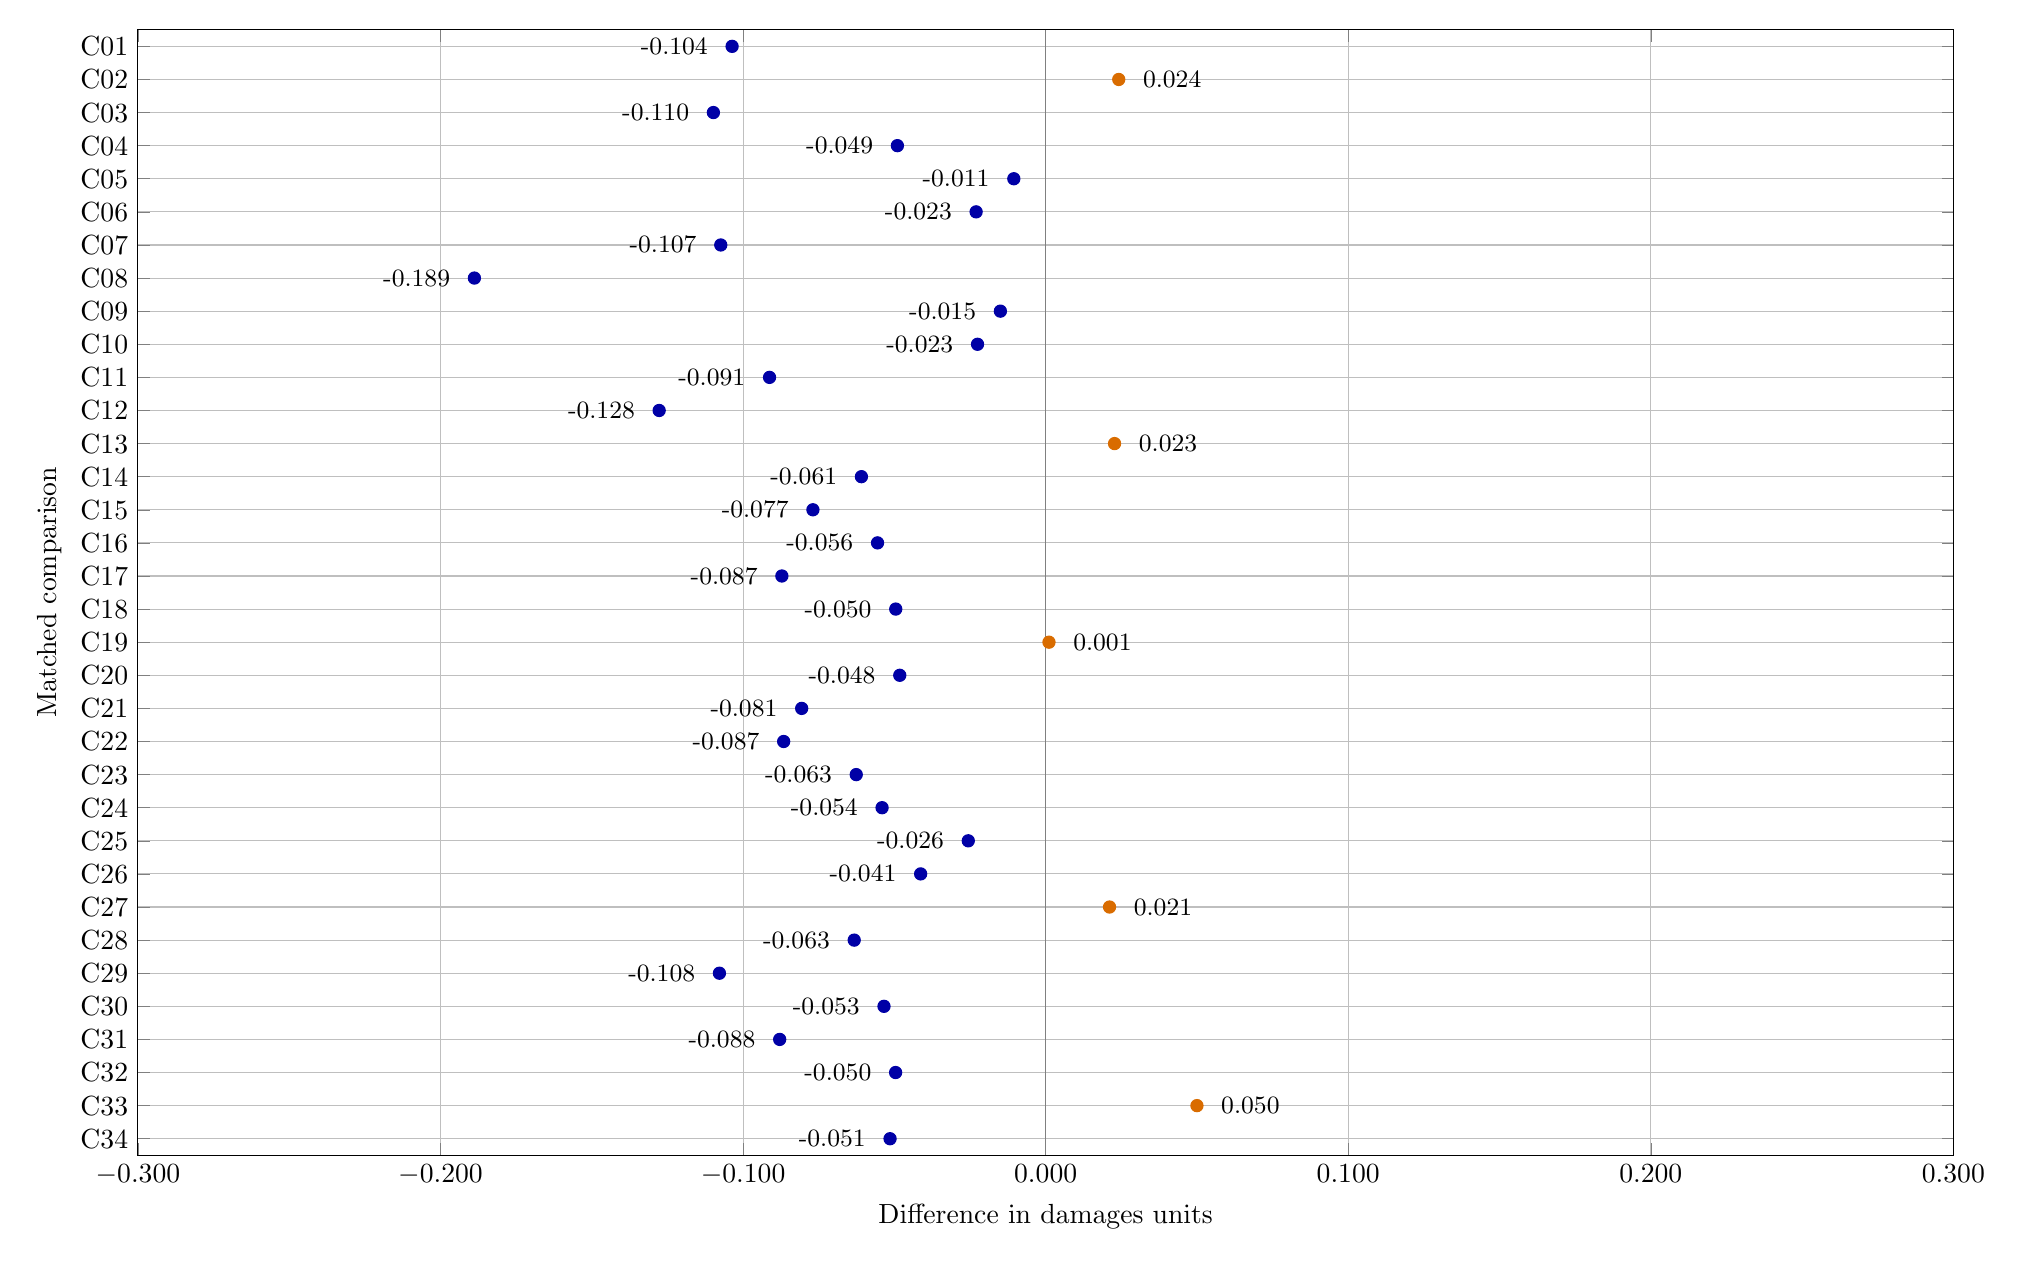
\begin{tikzpicture}\begin{axis}[width=9.7in,height=6.25in,
xmin=-0.30000000000000004,xmax=0.30000000000000004,ymin=.5,ymax=34.5,y dir=reverse,
ytick={1,2,3,4,5,6,7,8,9,10,11,12,13,14,15,16,17,18,19,20,21,22,23,24,25,26,27,28,29,30,31,32,33,34},
yticklabels={C01,C02,C03,C04,C05,C06,C07,C08,C09,C10,C11,C12,C13,C14,C15,C16,C17,C18,C19,C20,C21,C22,C23,C24,C25,C26,C27,C28,C29,C30,C31,C32,C33,C34},
xtick={-0.30000000000000004,-0.20000000000000001,-0.10000000000000001,0,0.10000000000000001,0.20000000000000001,0.30000000000000004},
xticklabel style={/pgf/number format/fixed,/pgf/number format/precision=3,/pgf/number format/fixed zerofill},
xlabel={Difference in damages units},ylabel={Matched comparison},grid=major,clip=false]
\addplot[gray,thin] coordinates {(0,.5) (0,34.5)};
\addplot[only marks,mark=*,mark size=2.2pt,color=blue!65!black] coordinates {(-0.10363554357912552,1)};
\node[font=\small,anchor=east] at (axis cs:-0.10843554357912552,1) {-0.104};
\addplot[only marks,mark=*,mark size=2.2pt,color=orange!85!black] coordinates {(0.024150598060490525,2)};
\node[font=\small,anchor=west] at (axis cs:0.028950598060490523,2) {0.024};
\addplot[only marks,mark=*,mark size=2.2pt,color=blue!65!black] coordinates {(-0.10981703622780264,3)};
\node[font=\small,anchor=east] at (axis cs:-0.11461703622780264,3) {-0.110};
\addplot[only marks,mark=*,mark size=2.2pt,color=blue!65!black] coordinates {(-0.049007242444649185,4)};
\node[font=\small,anchor=east] at (axis cs:-0.053807242444649184,4) {-0.049};
\addplot[only marks,mark=*,mark size=2.2pt,color=blue!65!black] coordinates {(-0.01052808491981877,5)};
\node[font=\small,anchor=east] at (axis cs:-0.01532808491981877,5) {-0.011};
\addplot[only marks,mark=*,mark size=2.2pt,color=blue!65!black] coordinates {(-0.022985134736603241,6)};
\node[font=\small,anchor=east] at (axis cs:-0.02778513473660324,6) {-0.023};
\addplot[only marks,mark=*,mark size=2.2pt,color=blue!65!black] coordinates {(-0.10737617222809839,7)};
\node[font=\small,anchor=east] at (axis cs:-0.11217617222809839,7) {-0.107};
\addplot[only marks,mark=*,mark size=2.2pt,color=blue!65!black] coordinates {(-0.18880309653801514,8)};
\node[font=\small,anchor=east] at (axis cs:-0.19360309653801513,8) {-0.189};
\addplot[only marks,mark=*,mark size=2.2pt,color=blue!65!black] coordinates {(-0.014967508501123356,9)};
\node[font=\small,anchor=east] at (axis cs:-0.019767508501123354,9) {-0.015};
\addplot[only marks,mark=*,mark size=2.2pt,color=blue!65!black] coordinates {(-0.022516437431737757,10)};
\node[font=\small,anchor=east] at (axis cs:-0.027316437431737756,10) {-0.023};
\addplot[only marks,mark=*,mark size=2.2pt,color=blue!65!black] coordinates {(-0.091262529613463261,11)};
\node[font=\small,anchor=east] at (axis cs:-0.09606252961346326,11) {-0.091};
\addplot[only marks,mark=*,mark size=2.2pt,color=blue!65!black] coordinates {(-0.12773660444100096,12)};
\node[font=\small,anchor=east] at (axis cs:-0.13253660444100096,12) {-0.128};
\addplot[only marks,mark=*,mark size=2.2pt,color=orange!85!black] coordinates {(0.022765606415648065,13)};
\node[font=\small,anchor=west] at (axis cs:0.027565606415648064,13) {0.023};
\addplot[only marks,mark=*,mark size=2.2pt,color=blue!65!black] coordinates {(-0.060893830898703316,14)};
\node[font=\small,anchor=east] at (axis cs:-0.065693830898703315,14) {-0.061};
\addplot[only marks,mark=*,mark size=2.2pt,color=blue!65!black] coordinates {(-0.076924419698949503,15)};
\node[font=\small,anchor=east] at (axis cs:-0.081724419698949502,15) {-0.077};
\addplot[only marks,mark=*,mark size=2.2pt,color=blue!65!black] coordinates {(-0.055563021152630648,16)};
\node[font=\small,anchor=east] at (axis cs:-0.060363021152630647,16) {-0.056};
\addplot[only marks,mark=*,mark size=2.2pt,color=blue!65!black] coordinates {(-0.087184681638329514,17)};
\node[font=\small,anchor=east] at (axis cs:-0.091984681638329513,17) {-0.087};
\addplot[only marks,mark=*,mark size=2.2pt,color=blue!65!black] coordinates {(-0.049548841822493195,18)};
\node[font=\small,anchor=east] at (axis cs:-0.054348841822493194,18) {-0.050};
\addplot[only marks,mark=*,mark size=2.2pt,color=orange!85!black] coordinates {(0.0010958830322607138,19)};
\node[font=\small,anchor=west] at (axis cs:0.0058958830322607143,19) {0.001};
\addplot[only marks,mark=*,mark size=2.2pt,color=blue!65!black] coordinates {(-0.048222675342763366,20)};
\node[font=\small,anchor=east] at (axis cs:-0.053022675342763365,20) {-0.048};
\addplot[only marks,mark=*,mark size=2.2pt,color=blue!65!black] coordinates {(-0.080633528915936198,21)};
\node[font=\small,anchor=east] at (axis cs:-0.085433528915936197,21) {-0.081};
\addplot[only marks,mark=*,mark size=2.2pt,color=blue!65!black] coordinates {(-0.086586583859167454,22)};
\node[font=\small,anchor=east] at (axis cs:-0.091386583859167453,22) {-0.087};
\addplot[only marks,mark=*,mark size=2.2pt,color=blue!65!black] coordinates {(-0.06260603280679955,23)};
\node[font=\small,anchor=east] at (axis cs:-0.067406032806799548,23) {-0.063};
\addplot[only marks,mark=*,mark size=2.2pt,color=blue!65!black] coordinates {(-0.054069368732011819,24)};
\node[font=\small,anchor=east] at (axis cs:-0.058869368732011818,24) {-0.054};
\addplot[only marks,mark=*,mark size=2.2pt,color=blue!65!black] coordinates {(-0.025578905042923594,25)};
\node[font=\small,anchor=east] at (axis cs:-0.030378905042923593,25) {-0.026};
\addplot[only marks,mark=*,mark size=2.2pt,color=blue!65!black] coordinates {(-0.041313878931703324,26)};
\node[font=\small,anchor=east] at (axis cs:-0.046113878931703323,26) {-0.041};
\addplot[only marks,mark=*,mark size=2.2pt,color=orange!85!black] coordinates {(0.021108753344544262,27)};
\node[font=\small,anchor=west] at (axis cs:0.025908753344544261,27) {0.021};
\addplot[only marks,mark=*,mark size=2.2pt,color=blue!65!black] coordinates {(-0.063280602738303965,28)};
\node[font=\small,anchor=east] at (axis cs:-0.068080602738303964,28) {-0.063};
\addplot[only marks,mark=*,mark size=2.2pt,color=blue!65!black] coordinates {(-0.10782127679282348,29)};
\node[font=\small,anchor=east] at (axis cs:-0.11262127679282348,29) {-0.108};
\addplot[only marks,mark=*,mark size=2.2pt,color=blue!65!black] coordinates {(-0.053431247185750902,30)};
\node[font=\small,anchor=east] at (axis cs:-0.058231247185750901,30) {-0.053};
\addplot[only marks,mark=*,mark size=2.2pt,color=blue!65!black] coordinates {(-0.087905510694434669,31)};
\node[font=\small,anchor=east] at (axis cs:-0.092705510694434667,31) {-0.088};
\addplot[only marks,mark=*,mark size=2.2pt,color=blue!65!black] coordinates {(-0.049594872454163913,32)};
\node[font=\small,anchor=east] at (axis cs:-0.054394872454163912,32) {-0.050};
\addplot[only marks,mark=*,mark size=2.2pt,color=orange!85!black] coordinates {(0.049999999999999989,33)};
\node[font=\small,anchor=west] at (axis cs:0.054799999999999988,33) {0.050};
\addplot[only marks,mark=*,mark size=2.2pt,color=blue!65!black] coordinates {(-0.051430460135435924,34)};
\node[font=\small,anchor=east] at (axis cs:-0.056230460135435922,34) {-0.051};
\end{axis}\end{tikzpicture}\end{center}
\newpage
{\LARGE\bfseries Nonliable defendant burden}\par\smallskip
British minus American, using unrounded values. Codes identify the preceding matched-comparison table. Blue: negative; orange: positive. This is one monetary measure, not a combined policy ranking.\par\medskip
\begin{center}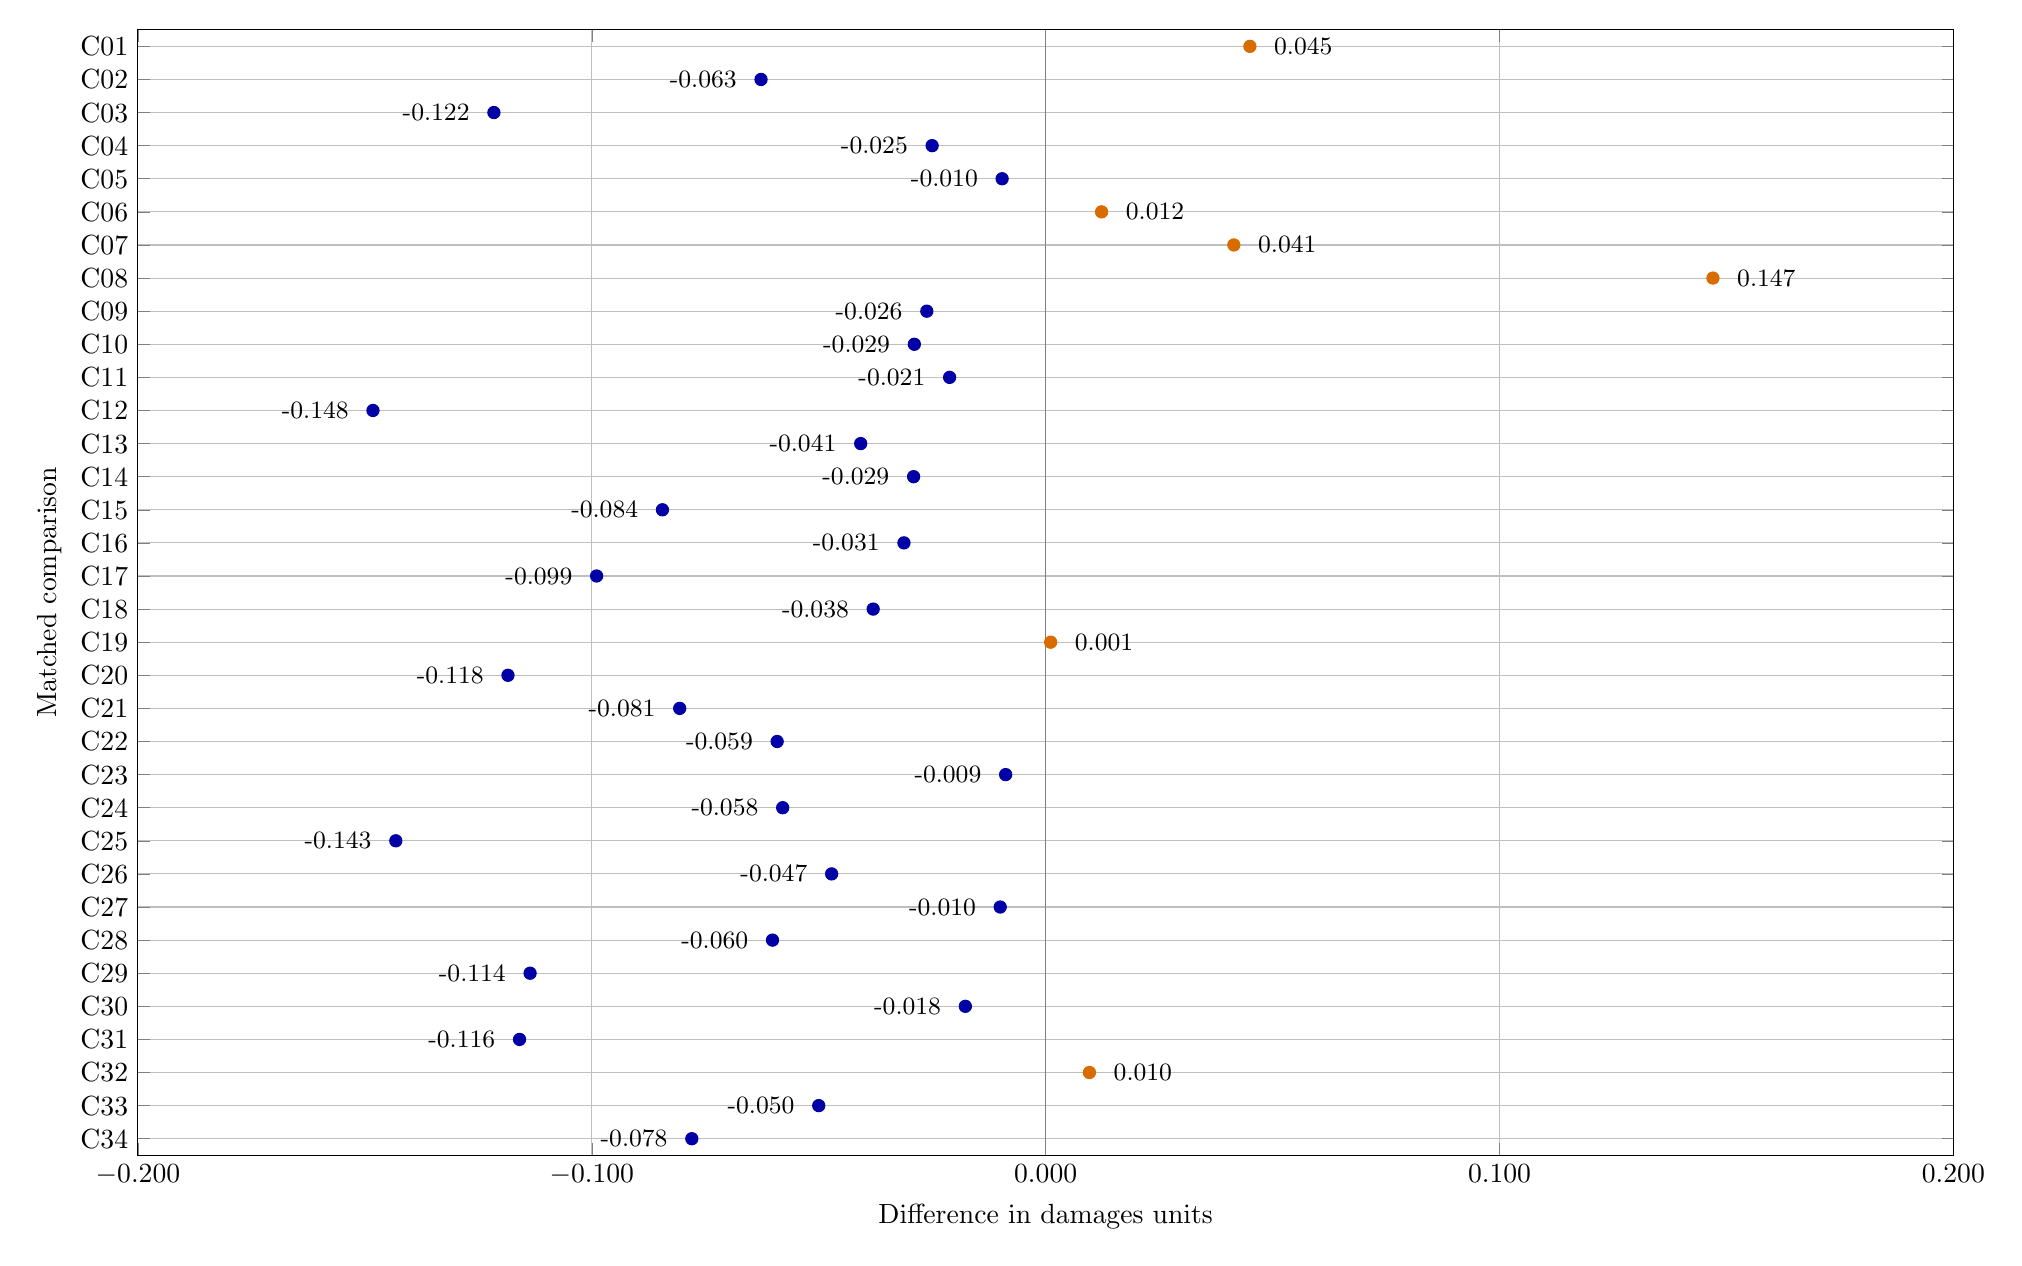
\begin{tikzpicture}\begin{axis}[width=9.7in,height=6.25in,
xmin=-0.20000000000000001,xmax=0.20000000000000001,ymin=.5,ymax=34.5,y dir=reverse,
ytick={1,2,3,4,5,6,7,8,9,10,11,12,13,14,15,16,17,18,19,20,21,22,23,24,25,26,27,28,29,30,31,32,33,34},
yticklabels={C01,C02,C03,C04,C05,C06,C07,C08,C09,C10,C11,C12,C13,C14,C15,C16,C17,C18,C19,C20,C21,C22,C23,C24,C25,C26,C27,C28,C29,C30,C31,C32,C33,C34},
xtick={-0.20000000000000001,-0.10000000000000001,0,0.10000000000000001,0.20000000000000001},
xticklabel style={/pgf/number format/fixed,/pgf/number format/precision=3,/pgf/number format/fixed zerofill},
xlabel={Difference in damages units},ylabel={Matched comparison},grid=major,clip=false]
\addplot[gray,thin] coordinates {(0,.5) (0,34.5)};
\addplot[only marks,mark=*,mark size=2.2pt,color=orange!85!black] coordinates {(0.044995492360103972,1)};
\node[font=\small,anchor=west] at (axis cs:0.048195492360103974,1) {0.045};
\addplot[only marks,mark=*,mark size=2.2pt,color=blue!65!black] coordinates {(-0.062713837233121808,2)};
\node[font=\small,anchor=east] at (axis cs:-0.065913837233121803,2) {-0.063};
\addplot[only marks,mark=*,mark size=2.2pt,color=blue!65!black] coordinates {(-0.12157352969202007,3)};
\node[font=\small,anchor=east] at (axis cs:-0.12477352969202006,3) {-0.122};
\addplot[only marks,mark=*,mark size=2.2pt,color=blue!65!black] coordinates {(-0.025014419911815161,4)};
\node[font=\small,anchor=east] at (axis cs:-0.028214419911815163,4) {-0.025};
\addplot[only marks,mark=*,mark size=2.2pt,color=blue!65!black] coordinates {(-0.0095947548348327416,5)};
\node[font=\small,anchor=east] at (axis cs:-0.012794754834832741,5) {-0.010};
\addplot[only marks,mark=*,mark size=2.2pt,color=orange!85!black] coordinates {(0.012316147032209179,6)};
\node[font=\small,anchor=west] at (axis cs:0.015516147032209179,6) {0.012};
\addplot[only marks,mark=*,mark size=2.2pt,color=orange!85!black] coordinates {(0.041457070742456525,7)};
\node[font=\small,anchor=west] at (axis cs:0.044657070742456527,7) {0.041};
\addplot[only marks,mark=*,mark size=2.2pt,color=orange!85!black] coordinates {(0.14701750706411898,8)};
\node[font=\small,anchor=west] at (axis cs:0.15021750706411899,8) {0.147};
\addplot[only marks,mark=*,mark size=2.2pt,color=blue!65!black] coordinates {(-0.026187867725191438,9)};
\node[font=\small,anchor=east] at (axis cs:-0.02938786772519144,9) {-0.026};
\addplot[only marks,mark=*,mark size=2.2pt,color=blue!65!black] coordinates {(-0.028936740670121891,10)};
\node[font=\small,anchor=east] at (axis cs:-0.032136740670121892,10) {-0.029};
\addplot[only marks,mark=*,mark size=2.2pt,color=blue!65!black] coordinates {(-0.021164033037855523,11)};
\node[font=\small,anchor=east] at (axis cs:-0.024364033037855524,11) {-0.021};
\addplot[only marks,mark=*,mark size=2.2pt,color=blue!65!black] coordinates {(-0.14821487184862445,12)};
\node[font=\small,anchor=east] at (axis cs:-0.15141487184862445,12) {-0.148};
\addplot[only marks,mark=*,mark size=2.2pt,color=blue!65!black] coordinates {(-0.040755406483389683,13)};
\node[font=\small,anchor=east] at (axis cs:-0.043955406483389685,13) {-0.041};
\addplot[only marks,mark=*,mark size=2.2pt,color=blue!65!black] coordinates {(-0.029100016383116656,14)};
\node[font=\small,anchor=east] at (axis cs:-0.032300016383116657,14) {-0.029};
\addplot[only marks,mark=*,mark size=2.2pt,color=blue!65!black] coordinates {(-0.084440153300323478,15)};
\node[font=\small,anchor=east] at (axis cs:-0.087640153300323473,15) {-0.084};
\addplot[only marks,mark=*,mark size=2.2pt,color=blue!65!black] coordinates {(-0.03122934382645165,16)};
\node[font=\small,anchor=east] at (axis cs:-0.034429343826451651,16) {-0.031};
\addplot[only marks,mark=*,mark size=2.2pt,color=blue!65!black] coordinates {(-0.098939686373884866,17)};
\node[font=\small,anchor=east] at (axis cs:-0.10213968637388486,17) {-0.099};
\addplot[only marks,mark=*,mark size=2.2pt,color=blue!65!black] coordinates {(-0.038006992197402362,18)};
\node[font=\small,anchor=east] at (axis cs:-0.041206992197402363,18) {-0.038};
\addplot[only marks,mark=*,mark size=2.2pt,color=orange!85!black] coordinates {(0.001097288225016313,19)};
\node[font=\small,anchor=west] at (axis cs:0.0042972882250163127,19) {0.001};
\addplot[only marks,mark=*,mark size=2.2pt,color=blue!65!black] coordinates {(-0.11847352315454412,20)};
\node[font=\small,anchor=east] at (axis cs:-0.12167352315454412,20) {-0.118};
\addplot[only marks,mark=*,mark size=2.2pt,color=blue!65!black] coordinates {(-0.080632631429531476,21)};
\node[font=\small,anchor=east] at (axis cs:-0.083832631429531471,21) {-0.081};
\addplot[only marks,mark=*,mark size=2.2pt,color=blue!65!black] coordinates {(-0.059164123308457085,22)};
\node[font=\small,anchor=east] at (axis cs:-0.062364123308457087,22) {-0.059};
\addplot[only marks,mark=*,mark size=2.2pt,color=blue!65!black] coordinates {(-0.008818710728063478,23)};
\node[font=\small,anchor=east] at (axis cs:-0.012018710728063478,23) {-0.009};
\addplot[only marks,mark=*,mark size=2.2pt,color=blue!65!black] coordinates {(-0.057944371151526564,24)};
\node[font=\small,anchor=east] at (axis cs:-0.061144371151526565,24) {-0.058};
\addplot[only marks,mark=*,mark size=2.2pt,color=blue!65!black] coordinates {(-0.14318381521938653,25)};
\node[font=\small,anchor=east] at (axis cs:-0.14638381521938654,25) {-0.143};
\addplot[only marks,mark=*,mark size=2.2pt,color=blue!65!black] coordinates {(-0.04715948860398228,26)};
\node[font=\small,anchor=east] at (axis cs:-0.050359488603982282,26) {-0.047};
\addplot[only marks,mark=*,mark size=2.2pt,color=blue!65!black] coordinates {(-0.010017849915039845,27)};
\node[font=\small,anchor=east] at (axis cs:-0.013217849915039845,27) {-0.010};
\addplot[only marks,mark=*,mark size=2.2pt,color=blue!65!black] coordinates {(-0.060187031377888417,28)};
\node[font=\small,anchor=east] at (axis cs:-0.063387031377888411,28) {-0.060};
\addplot[only marks,mark=*,mark size=2.2pt,color=blue!65!black] coordinates {(-0.11359575722097659,29)};
\node[font=\small,anchor=east] at (axis cs:-0.11679575722097658,29) {-0.114};
\addplot[only marks,mark=*,mark size=2.2pt,color=blue!65!black] coordinates {(-0.017696886231548054,30)};
\node[font=\small,anchor=east] at (axis cs:-0.020896886231548055,30) {-0.018};
\addplot[only marks,mark=*,mark size=2.2pt,color=blue!65!black] coordinates {(-0.11592430265019188,31)};
\node[font=\small,anchor=east] at (axis cs:-0.11912430265019187,31) {-0.116};
\addplot[only marks,mark=*,mark size=2.2pt,color=orange!85!black] coordinates {(0.0096371418147731813,32)};
\node[font=\small,anchor=west] at (axis cs:0.012837141814773181,32) {0.010};
\addplot[only marks,mark=*,mark size=2.2pt,color=blue!65!black] coordinates {(-0.049999999999999933,33)};
\node[font=\small,anchor=east] at (axis cs:-0.053199999999999935,33) {-0.050};
\addplot[only marks,mark=*,mark size=2.2pt,color=blue!65!black] coordinates {(-0.077960825350580715,34)};
\node[font=\small,anchor=east] at (axis cs:-0.081160825350580709,34) {-0.078};
\end{axis}\end{tikzpicture}\end{center}
\newpage
{\LARGE\bfseries Liable defendant excess burden}\par\smallskip
British minus American, using unrounded values. Codes identify the preceding matched-comparison table. Blue: negative; orange: positive. This is one monetary measure, not a combined policy ranking.\par\medskip
\begin{center}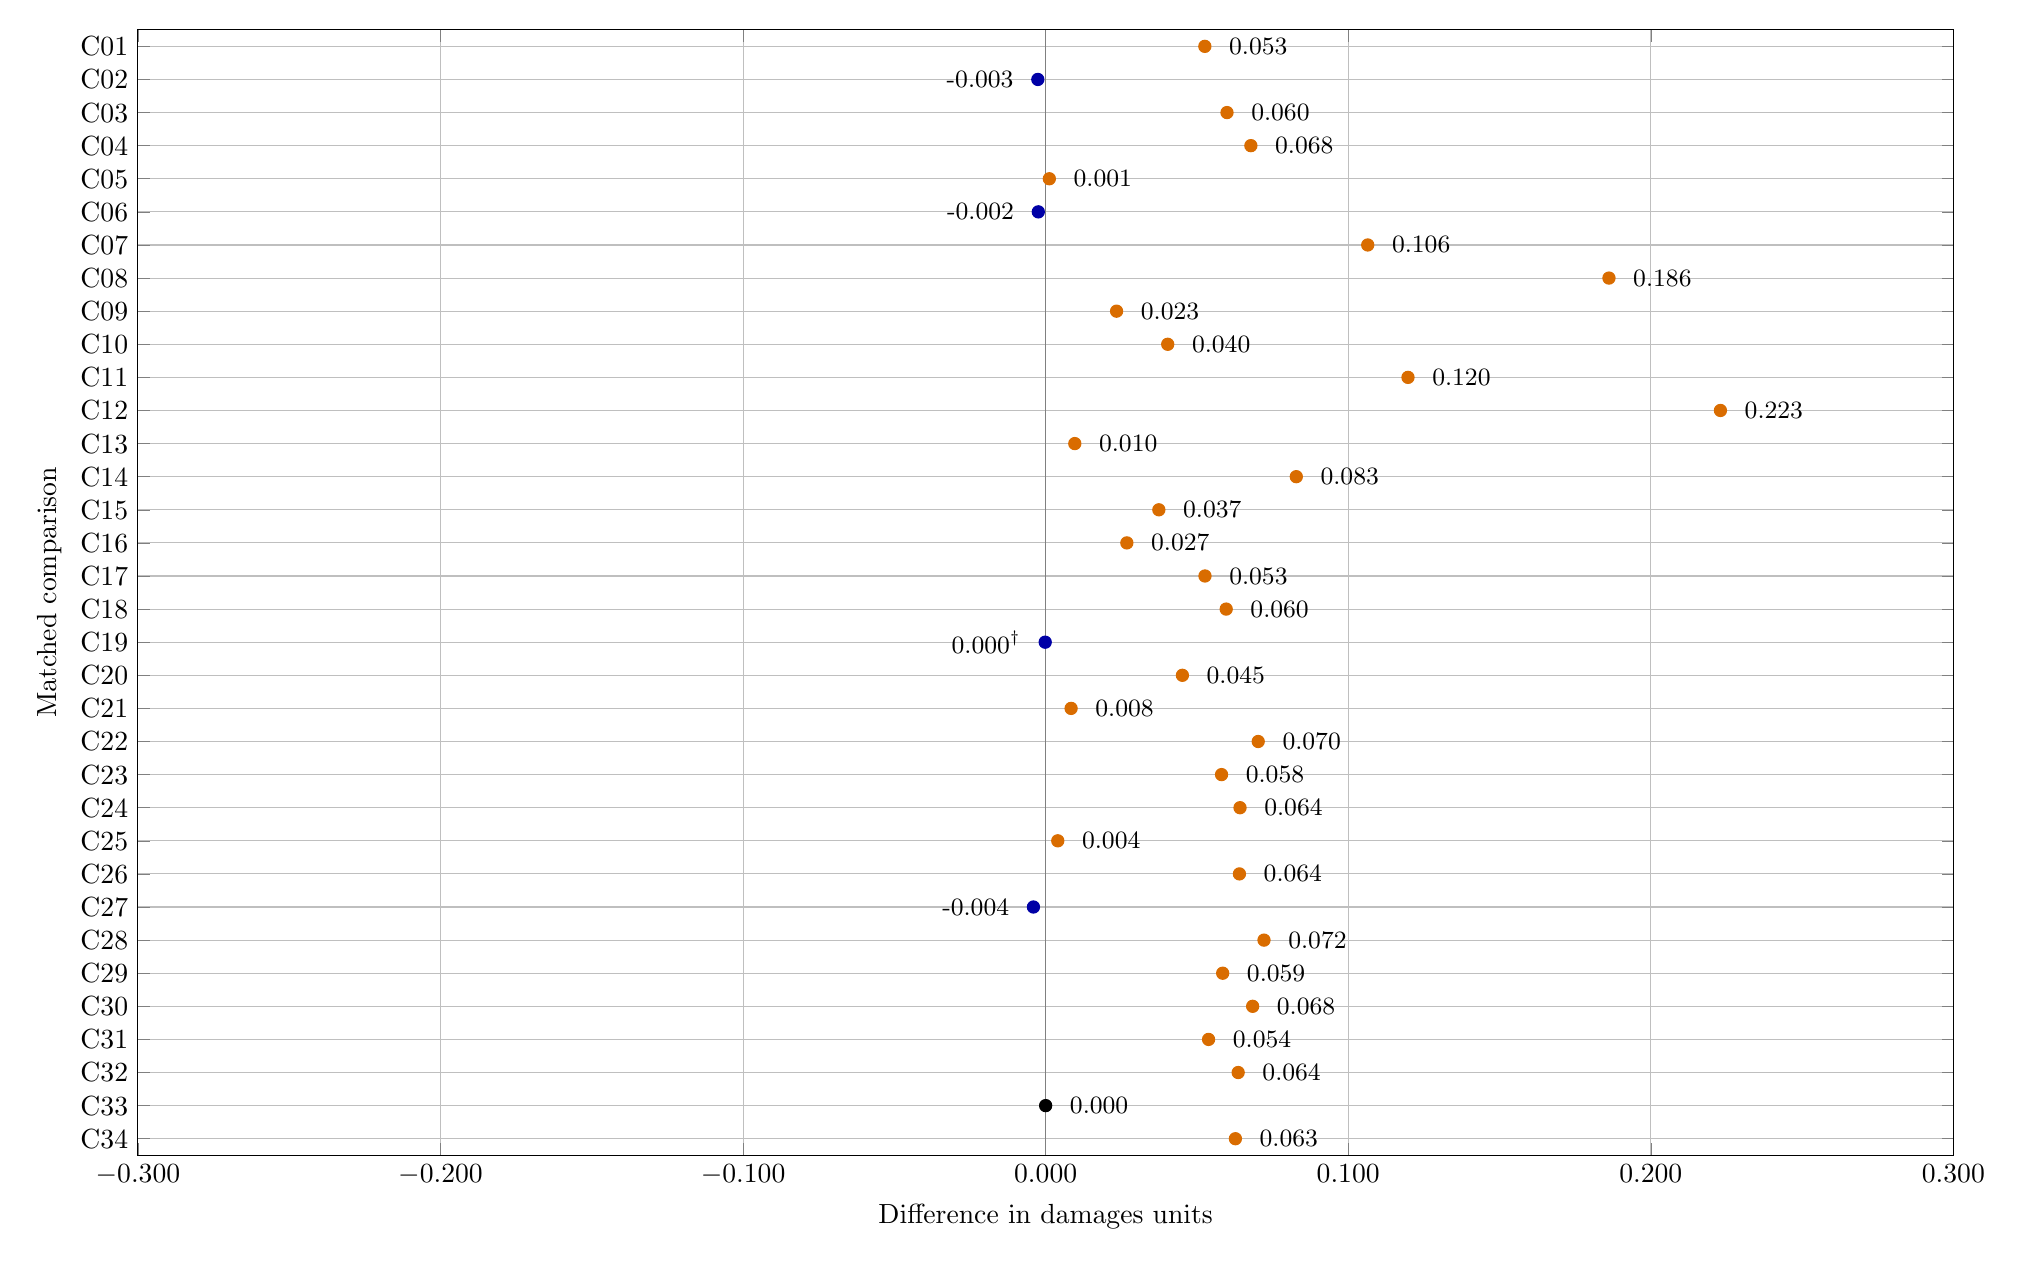
\begin{tikzpicture}\begin{axis}[width=9.7in,height=6.25in,
xmin=-0.30000000000000004,xmax=0.30000000000000004,ymin=.5,ymax=34.5,y dir=reverse,
ytick={1,2,3,4,5,6,7,8,9,10,11,12,13,14,15,16,17,18,19,20,21,22,23,24,25,26,27,28,29,30,31,32,33,34},
yticklabels={C01,C02,C03,C04,C05,C06,C07,C08,C09,C10,C11,C12,C13,C14,C15,C16,C17,C18,C19,C20,C21,C22,C23,C24,C25,C26,C27,C28,C29,C30,C31,C32,C33,C34},
xtick={-0.30000000000000004,-0.20000000000000001,-0.10000000000000001,0,0.10000000000000001,0.20000000000000001,0.30000000000000004},
xticklabel style={/pgf/number format/fixed,/pgf/number format/precision=3,/pgf/number format/fixed zerofill},
xlabel={Difference in damages units},ylabel={Matched comparison},grid=major,clip=false]
\addplot[gray,thin] coordinates {(0,.5) (0,34.5)};
\addplot[only marks,mark=*,mark size=2.2pt,color=orange!85!black] coordinates {(0.05260153458828952,1)};
\node[font=\small,anchor=west] at (axis cs:0.057401534588289518,1) {0.053};
\addplot[only marks,mark=*,mark size=2.2pt,color=blue!65!black] coordinates {(-0.0025886933427683757,2)};
\node[font=\small,anchor=east] at (axis cs:-0.0073886933427683762,2) {-0.003};
\addplot[only marks,mark=*,mark size=2.2pt,color=orange!85!black] coordinates {(0.059927319181926238,3)};
\node[font=\small,anchor=west] at (axis cs:0.064727319181926243,3) {0.060};
\addplot[only marks,mark=*,mark size=2.2pt,color=orange!85!black] coordinates {(0.067817804039225466,4)};
\node[font=\small,anchor=west] at (axis cs:0.072617804039225464,4) {0.068};
\addplot[only marks,mark=*,mark size=2.2pt,color=orange!85!black] coordinates {(0.0012152185572328104,5)};
\node[font=\small,anchor=west] at (axis cs:0.0060152185572328112,5) {0.001};
\addplot[only marks,mark=*,mark size=2.2pt,color=blue!65!black] coordinates {(-0.0024314338143659273,6)};
\node[font=\small,anchor=east] at (axis cs:-0.0072314338143659278,6) {-0.002};
\addplot[only marks,mark=*,mark size=2.2pt,color=orange!85!black] coordinates {(0.10643781203430044,7)};
\node[font=\small,anchor=west] at (axis cs:0.11123781203430044,7) {0.106};
\addplot[only marks,mark=*,mark size=2.2pt,color=orange!85!black] coordinates {(0.18616419144849161,8)};
\node[font=\small,anchor=west] at (axis cs:0.19096419144849161,8) {0.186};
\addplot[only marks,mark=*,mark size=2.2pt,color=orange!85!black] coordinates {(0.023436538217528929,9)};
\node[font=\small,anchor=west] at (axis cs:0.028236538217528931,9) {0.023};
\addplot[only marks,mark=*,mark size=2.2pt,color=orange!85!black] coordinates {(0.040339677926364517,10)};
\node[font=\small,anchor=west] at (axis cs:0.045139677926364516,10) {0.040};
\addplot[only marks,mark=*,mark size=2.2pt,color=orange!85!black] coordinates {(0.11974491510531501,11)};
\node[font=\small,anchor=west] at (axis cs:0.12454491510531501,11) {0.120};
\addplot[only marks,mark=*,mark size=2.2pt,color=orange!85!black] coordinates {(0.22300450593401155,12)};
\node[font=\small,anchor=west] at (axis cs:0.22780450593401155,12) {0.223};
\addplot[only marks,mark=*,mark size=2.2pt,color=orange!85!black] coordinates {(0.0096250828294888423,13)};
\node[font=\small,anchor=west] at (axis cs:0.014425082829488843,13) {0.010};
\addplot[only marks,mark=*,mark size=2.2pt,color=orange!85!black] coordinates {(0.082827799834756063,14)};
\node[font=\small,anchor=west] at (axis cs:0.087627799834756062,14) {0.083};
\addplot[only marks,mark=*,mark size=2.2pt,color=orange!85!black] coordinates {(0.03740598360234141,15)};
\node[font=\small,anchor=west] at (axis cs:0.042205983602341408,15) {0.037};
\addplot[only marks,mark=*,mark size=2.2pt,color=orange!85!black] coordinates {(0.026828295410183896,16)};
\node[font=\small,anchor=west] at (axis cs:0.031628295410183895,16) {0.027};
\addplot[only marks,mark=*,mark size=2.2pt,color=orange!85!black] coordinates {(0.052653895353329511,17)};
\node[font=\small,anchor=west] at (axis cs:0.057453895353329509,17) {0.053};
\addplot[only marks,mark=*,mark size=2.2pt,color=orange!85!black] coordinates {(0.059660003257428609,18)};
\node[font=\small,anchor=west] at (axis cs:0.064460003257428608,18) {0.060};
\addplot[only marks,mark=*,mark size=2.2pt,color=blue!65!black] coordinates {(-0.0001536537207122322,19)};
\node[font=\small,anchor=east] at (axis cs:-0.0049536537207122327,19) {0.000$^{\dagger}$};
\addplot[only marks,mark=*,mark size=2.2pt,color=orange!85!black] coordinates {(0.045189302457865288,20)};
\node[font=\small,anchor=west] at (axis cs:0.049989302457865287,20) {0.045};
\addplot[only marks,mark=*,mark size=2.2pt,color=orange!85!black] coordinates {(0.008405705413331202,21)};
\node[font=\small,anchor=west] at (axis cs:0.013205705413331202,21) {0.008};
\addplot[only marks,mark=*,mark size=2.2pt,color=orange!85!black] coordinates {(0.070244270461253727,22)};
\node[font=\small,anchor=west] at (axis cs:0.075044270461253726,22) {0.070};
\addplot[only marks,mark=*,mark size=2.2pt,color=orange!85!black] coordinates {(0.058126270443520658,23)};
\node[font=\small,anchor=west] at (axis cs:0.062926270443520657,23) {0.058};
\addplot[only marks,mark=*,mark size=2.2pt,color=orange!85!black] coordinates {(0.064233762769178221,24)};
\node[font=\small,anchor=west] at (axis cs:0.06903376276917822,24) {0.064};
\addplot[only marks,mark=*,mark size=2.2pt,color=orange!85!black] coordinates {(0.0040024846168041552,25)};
\node[font=\small,anchor=west] at (axis cs:0.0088024846168041557,25) {0.004};
\addplot[only marks,mark=*,mark size=2.2pt,color=orange!85!black] coordinates {(0.064034996516269135,26)};
\node[font=\small,anchor=west] at (axis cs:0.068834996516269134,26) {0.064};
\addplot[only marks,mark=*,mark size=2.2pt,color=blue!65!black] coordinates {(-0.0040449676705026751,27)};
\node[font=\small,anchor=east] at (axis cs:-0.0088449676705026764,27) {-0.004};
\addplot[only marks,mark=*,mark size=2.2pt,color=orange!85!black] coordinates {(0.072158516069748352,28)};
\node[font=\small,anchor=west] at (axis cs:0.076958516069748351,28) {0.072};
\addplot[only marks,mark=*,mark size=2.2pt,color=orange!85!black] coordinates {(0.058504619422193184,29)};
\node[font=\small,anchor=west] at (axis cs:0.06330461942219319,29) {0.059};
\addplot[only marks,mark=*,mark size=2.2pt,color=orange!85!black] coordinates {(0.068404750164004241,30)};
\node[font=\small,anchor=west] at (axis cs:0.07320475016400424,30) {0.068};
\addplot[only marks,mark=*,mark size=2.2pt,color=orange!85!black] coordinates {(0.053837338194957271,31)};
\node[font=\small,anchor=west] at (axis cs:0.05863733819495727,31) {0.054};
\addplot[only marks,mark=*,mark size=2.2pt,color=orange!85!black] coordinates {(0.063620030492404556,32)};
\node[font=\small,anchor=west] at (axis cs:0.068420030492404554,32) {0.064};
\addplot[only marks,mark=*,mark size=2.2pt,color=black] coordinates {(0,33)};
\node[font=\small,anchor=west] at (axis cs:0.0048000000000000004,33) {0.000};
\addplot[only marks,mark=*,mark size=2.2pt,color=orange!85!black] coordinates {(0.062704662165553426,34)};
\node[font=\small,anchor=west] at (axis cs:0.067504662165553425,34) {0.063};
\end{axis}\end{tikzpicture}\end{center}
\newpage
{\LARGE\bfseries Gross outcome error}\par\smallskip
British minus American, using unrounded values. Codes identify the preceding matched-comparison table. Blue: negative; orange: positive. This is one monetary measure, not a combined policy ranking.\par\medskip
\begin{center}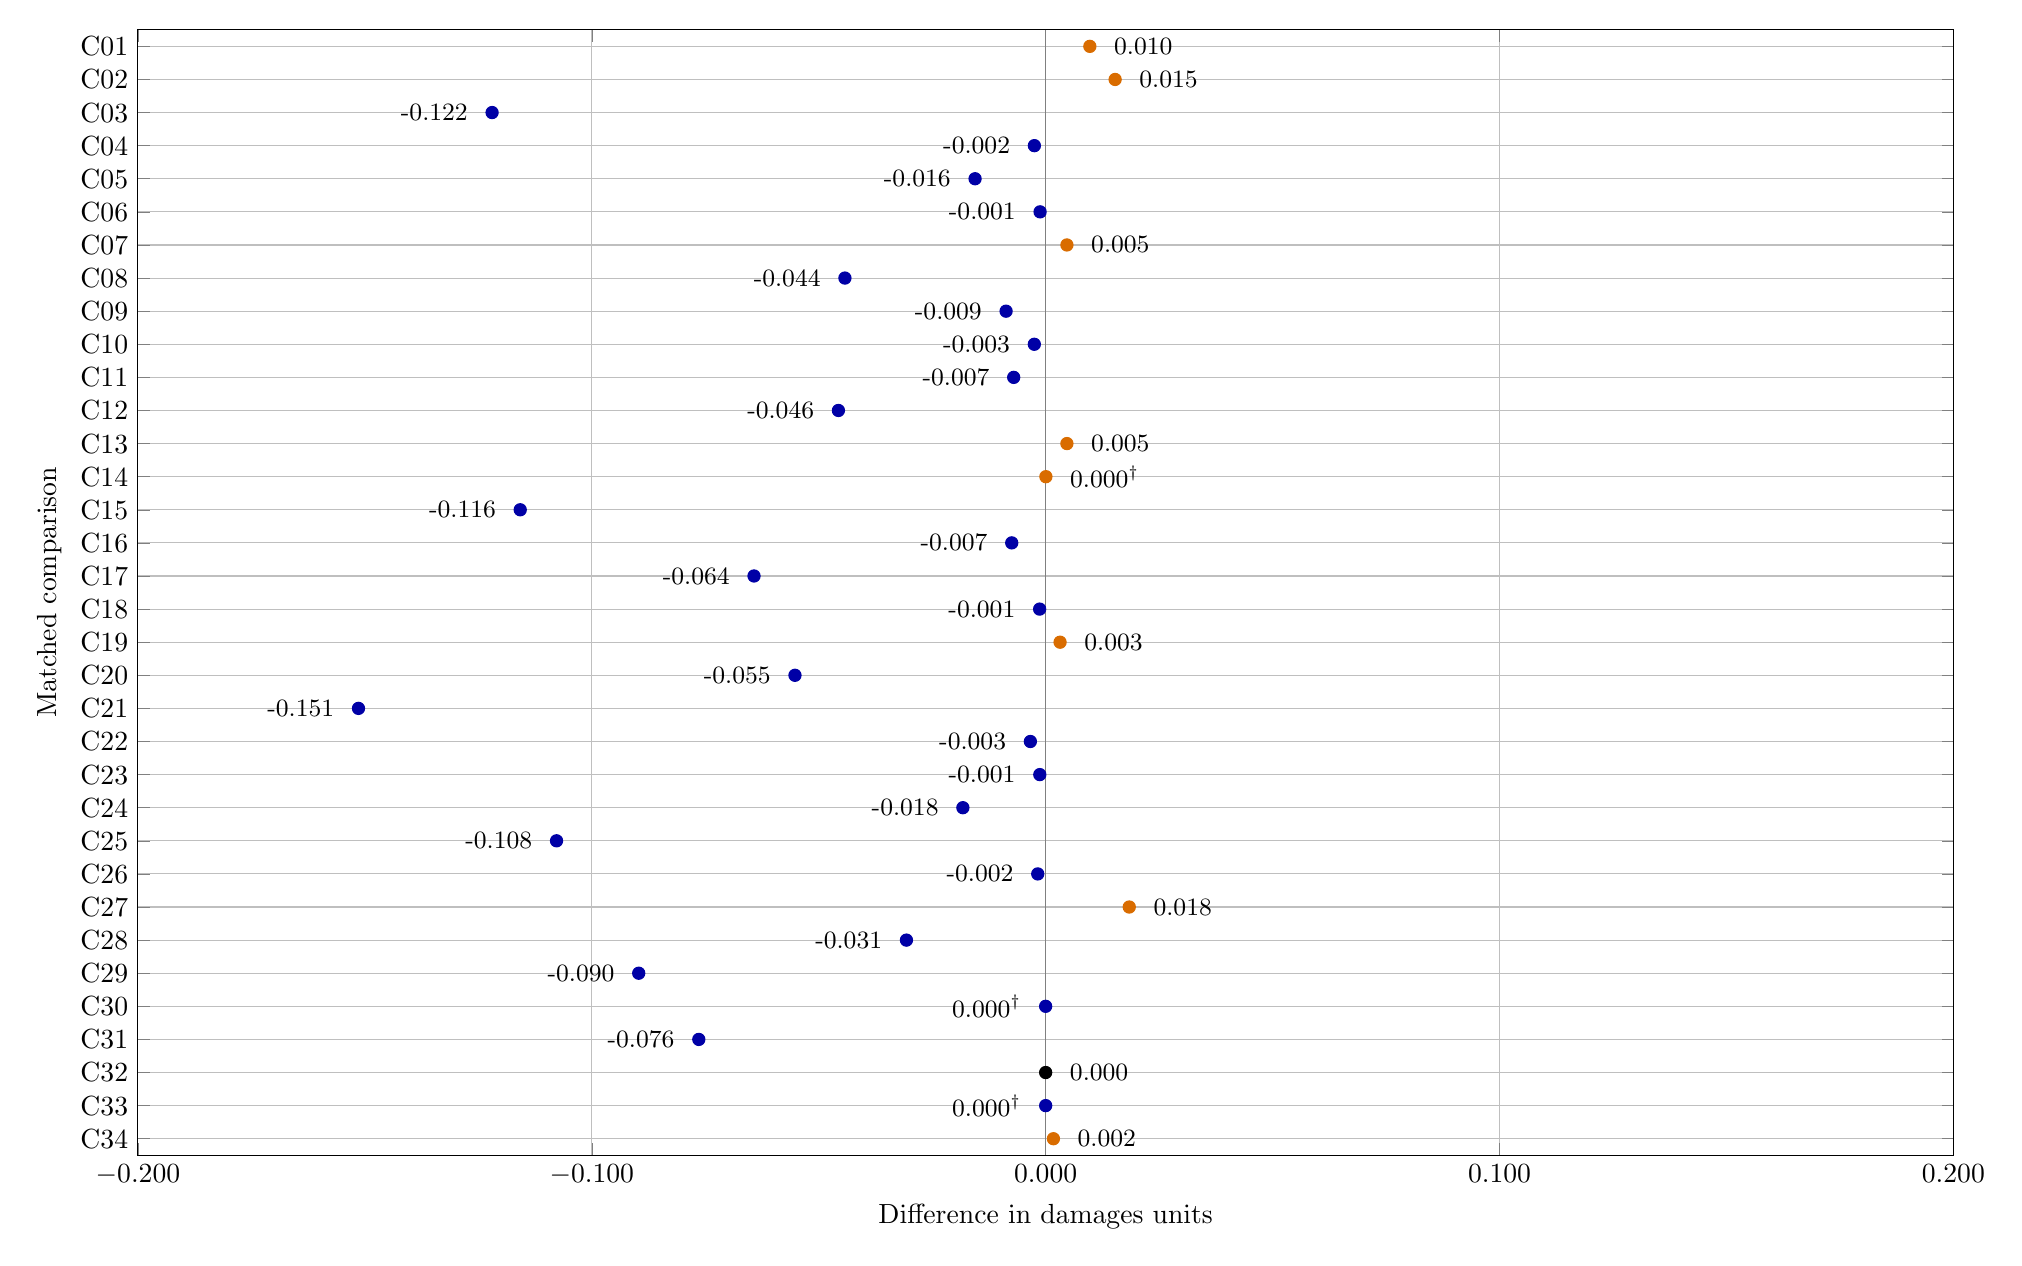
\begin{tikzpicture}\begin{axis}[width=9.7in,height=6.25in,
xmin=-0.20000000000000001,xmax=0.20000000000000001,ymin=.5,ymax=34.5,y dir=reverse,
ytick={1,2,3,4,5,6,7,8,9,10,11,12,13,14,15,16,17,18,19,20,21,22,23,24,25,26,27,28,29,30,31,32,33,34},
yticklabels={C01,C02,C03,C04,C05,C06,C07,C08,C09,C10,C11,C12,C13,C14,C15,C16,C17,C18,C19,C20,C21,C22,C23,C24,C25,C26,C27,C28,C29,C30,C31,C32,C33,C34},
xtick={-0.20000000000000001,-0.10000000000000001,0,0.10000000000000001,0.20000000000000001},
xticklabel style={/pgf/number format/fixed,/pgf/number format/precision=3,/pgf/number format/fixed zerofill},
xlabel={Difference in damages units},ylabel={Matched comparison},grid=major,clip=false]
\addplot[gray,thin] coordinates {(0,.5) (0,34.5)};
\addplot[only marks,mark=*,mark size=2.2pt,color=orange!85!black] coordinates {(0.0097289872728082982,1)};
\node[font=\small,anchor=west] at (axis cs:0.012928987272808298,1) {0.010};
\addplot[only marks,mark=*,mark size=2.2pt,color=orange!85!black] coordinates {(0.01530383118113815,2)};
\node[font=\small,anchor=west] at (axis cs:0.018503831181138151,2) {0.015};
\addplot[only marks,mark=*,mark size=2.2pt,color=blue!65!black] coordinates {(-0.12197050688935301,3)};
\node[font=\small,anchor=east] at (axis cs:-0.12517050688935302,3) {-0.122};
\addplot[only marks,mark=*,mark size=2.2pt,color=blue!65!black] coordinates {(-0.0024911718702095298,4)};
\node[font=\small,anchor=east] at (axis cs:-0.0056911718702095295,4) {-0.002};
\addplot[only marks,mark=*,mark size=2.2pt,color=blue!65!black] coordinates {(-0.015556011394898206,5)};
\node[font=\small,anchor=east] at (axis cs:-0.018756011394898207,5) {-0.016};
\addplot[only marks,mark=*,mark size=2.2pt,color=blue!65!black] coordinates {(-0.0012329689404725896,6)};
\node[font=\small,anchor=east] at (axis cs:-0.0044329689404725894,6) {-0.001};
\addplot[only marks,mark=*,mark size=2.2pt,color=orange!85!black] coordinates {(0.0046787259717936402,7)};
\node[font=\small,anchor=west] at (axis cs:0.00787872597179364,7) {0.005};
\addplot[only marks,mark=*,mark size=2.2pt,color=blue!65!black] coordinates {(-0.044232905345037377,8)};
\node[font=\small,anchor=east] at (axis cs:-0.047432905345037378,8) {-0.044};
\addplot[only marks,mark=*,mark size=2.2pt,color=blue!65!black] coordinates {(-0.0087231266591821788,9)};
\node[font=\small,anchor=east] at (axis cs:-0.011923126659182178,9) {-0.009};
\addplot[only marks,mark=*,mark size=2.2pt,color=blue!65!black] coordinates {(-0.0025041119619207963,10)};
\node[font=\small,anchor=east] at (axis cs:-0.005704111961920796,10) {-0.003};
\addplot[only marks,mark=*,mark size=2.2pt,color=blue!65!black] coordinates {(-0.0070412321856996307,11)};
\node[font=\small,anchor=east] at (axis cs:-0.01024123218569963,11) {-0.007};
\addplot[only marks,mark=*,mark size=2.2pt,color=blue!65!black] coordinates {(-0.045667061482326354,12)};
\node[font=\small,anchor=east] at (axis cs:-0.048867061482326356,12) {-0.046};
\addplot[only marks,mark=*,mark size=2.2pt,color=orange!85!black] coordinates {(0.0046782363398663596,13)};
\node[font=\small,anchor=west] at (axis cs:0.0078782363398663593,13) {0.005};
\addplot[only marks,mark=*,mark size=2.2pt,color=orange!85!black] coordinates {(4.6246129753901855e-05,14)};
\node[font=\small,anchor=west] at (axis cs:0.003246246129753902,14) {0.000$^{\dagger}$};
\addplot[only marks,mark=*,mark size=2.2pt,color=blue!65!black] coordinates {(-0.11577283807861538,15)};
\node[font=\small,anchor=east] at (axis cs:-0.11897283807861538,15) {-0.116};
\addplot[only marks,mark=*,mark size=2.2pt,color=blue!65!black] coordinates {(-0.0074745573852557645,16)};
\node[font=\small,anchor=east] at (axis cs:-0.010674557385255764,16) {-0.007};
\addplot[only marks,mark=*,mark size=2.2pt,color=blue!65!black] coordinates {(-0.064260719830091184,17)};
\node[font=\small,anchor=east] at (axis cs:-0.067460719830091179,17) {-0.064};
\addplot[only marks,mark=*,mark size=2.2pt,color=blue!65!black] coordinates {(-0.001329303802082682,18)};
\node[font=\small,anchor=east] at (axis cs:-0.0045293038020826817,18) {-0.001};
\addplot[only marks,mark=*,mark size=2.2pt,color=orange!85!black] coordinates {(0.0031719090936168648,19)};
\node[font=\small,anchor=west] at (axis cs:0.0063719090936168645,19) {0.003};
\addplot[only marks,mark=*,mark size=2.2pt,color=blue!65!black] coordinates {(-0.055236729141312557,20)};
\node[font=\small,anchor=east] at (axis cs:-0.058436729141312559,20) {-0.055};
\addplot[only marks,mark=*,mark size=2.2pt,color=blue!65!black] coordinates {(-0.15140660737612555,21)};
\node[font=\small,anchor=east] at (axis cs:-0.15460660737612555,21) {-0.151};
\addplot[only marks,mark=*,mark size=2.2pt,color=blue!65!black] coordinates {(-0.0033689099476466311,22)};
\node[font=\small,anchor=east] at (axis cs:-0.0065689099476466308,22) {-0.003};
\addplot[only marks,mark=*,mark size=2.2pt,color=blue!65!black] coordinates {(-0.0012949764623835236,23)};
\node[font=\small,anchor=east] at (axis cs:-0.0044949764623835233,23) {-0.001};
\addplot[only marks,mark=*,mark size=2.2pt,color=blue!65!black] coordinates {(-0.018241023520261912,24)};
\node[font=\small,anchor=east] at (axis cs:-0.021441023520261913,24) {-0.018};
\addplot[only marks,mark=*,mark size=2.2pt,color=blue!65!black] coordinates {(-0.10777051648203212,25)};
\node[font=\small,anchor=east] at (axis cs:-0.11097051648203211,25) {-0.108};
\addplot[only marks,mark=*,mark size=2.2pt,color=blue!65!black] coordinates {(-0.0017446580551609414,26)};
\node[font=\small,anchor=east] at (axis cs:-0.0049446580551609411,26) {-0.002};
\addplot[only marks,mark=*,mark size=2.2pt,color=orange!85!black] coordinates {(0.018413406360196172,27)};
\node[font=\small,anchor=west] at (axis cs:0.021613406360196173,27) {0.018};
\addplot[only marks,mark=*,mark size=2.2pt,color=blue!65!black] coordinates {(-0.030679506457634398,28)};
\node[font=\small,anchor=east] at (axis cs:-0.033879506457634399,28) {-0.031};
\addplot[only marks,mark=*,mark size=2.2pt,color=blue!65!black] coordinates {(-0.08966332524129017,29)};
\node[font=\small,anchor=east] at (axis cs:-0.092863325241290165,29) {-0.090};
\addplot[only marks,mark=*,mark size=2.2pt,color=blue!65!black] coordinates {(-6.340578446839551e-06,30)};
\node[font=\small,anchor=east] at (axis cs:-0.0032063405784468397,30) {0.000$^{\dagger}$};
\addplot[only marks,mark=*,mark size=2.2pt,color=blue!65!black] coordinates {(-0.076425550000381148,31)};
\node[font=\small,anchor=east] at (axis cs:-0.079625550000381143,31) {-0.076};
\addplot[only marks,mark=*,mark size=2.2pt,color=black] coordinates {(0,32)};
\node[font=\small,anchor=west] at (axis cs:0.0032000000000000002,32) {0.000};
\addplot[only marks,mark=*,mark size=2.2pt,color=blue!65!black] coordinates {(-2.2204460492503131e-16,33)};
\node[font=\small,anchor=east] at (axis cs:-0.0032000000000002222,33) {0.000$^{\dagger}$};
\addplot[only marks,mark=*,mark size=2.2pt,color=orange!85!black] coordinates {(0.0017032016959812601,34)};
\node[font=\small,anchor=west] at (axis cs:0.0049032016959812599,34) {0.002};
\end{axis}\end{tikzpicture}\end{center}
\newpage
{\LARGE\bfseries Real litigation expenditures}\par\smallskip
British minus American, using unrounded values. Codes identify the preceding matched-comparison table. Blue: negative; orange: positive. This is one monetary measure, not a combined policy ranking.\par\medskip
\begin{center}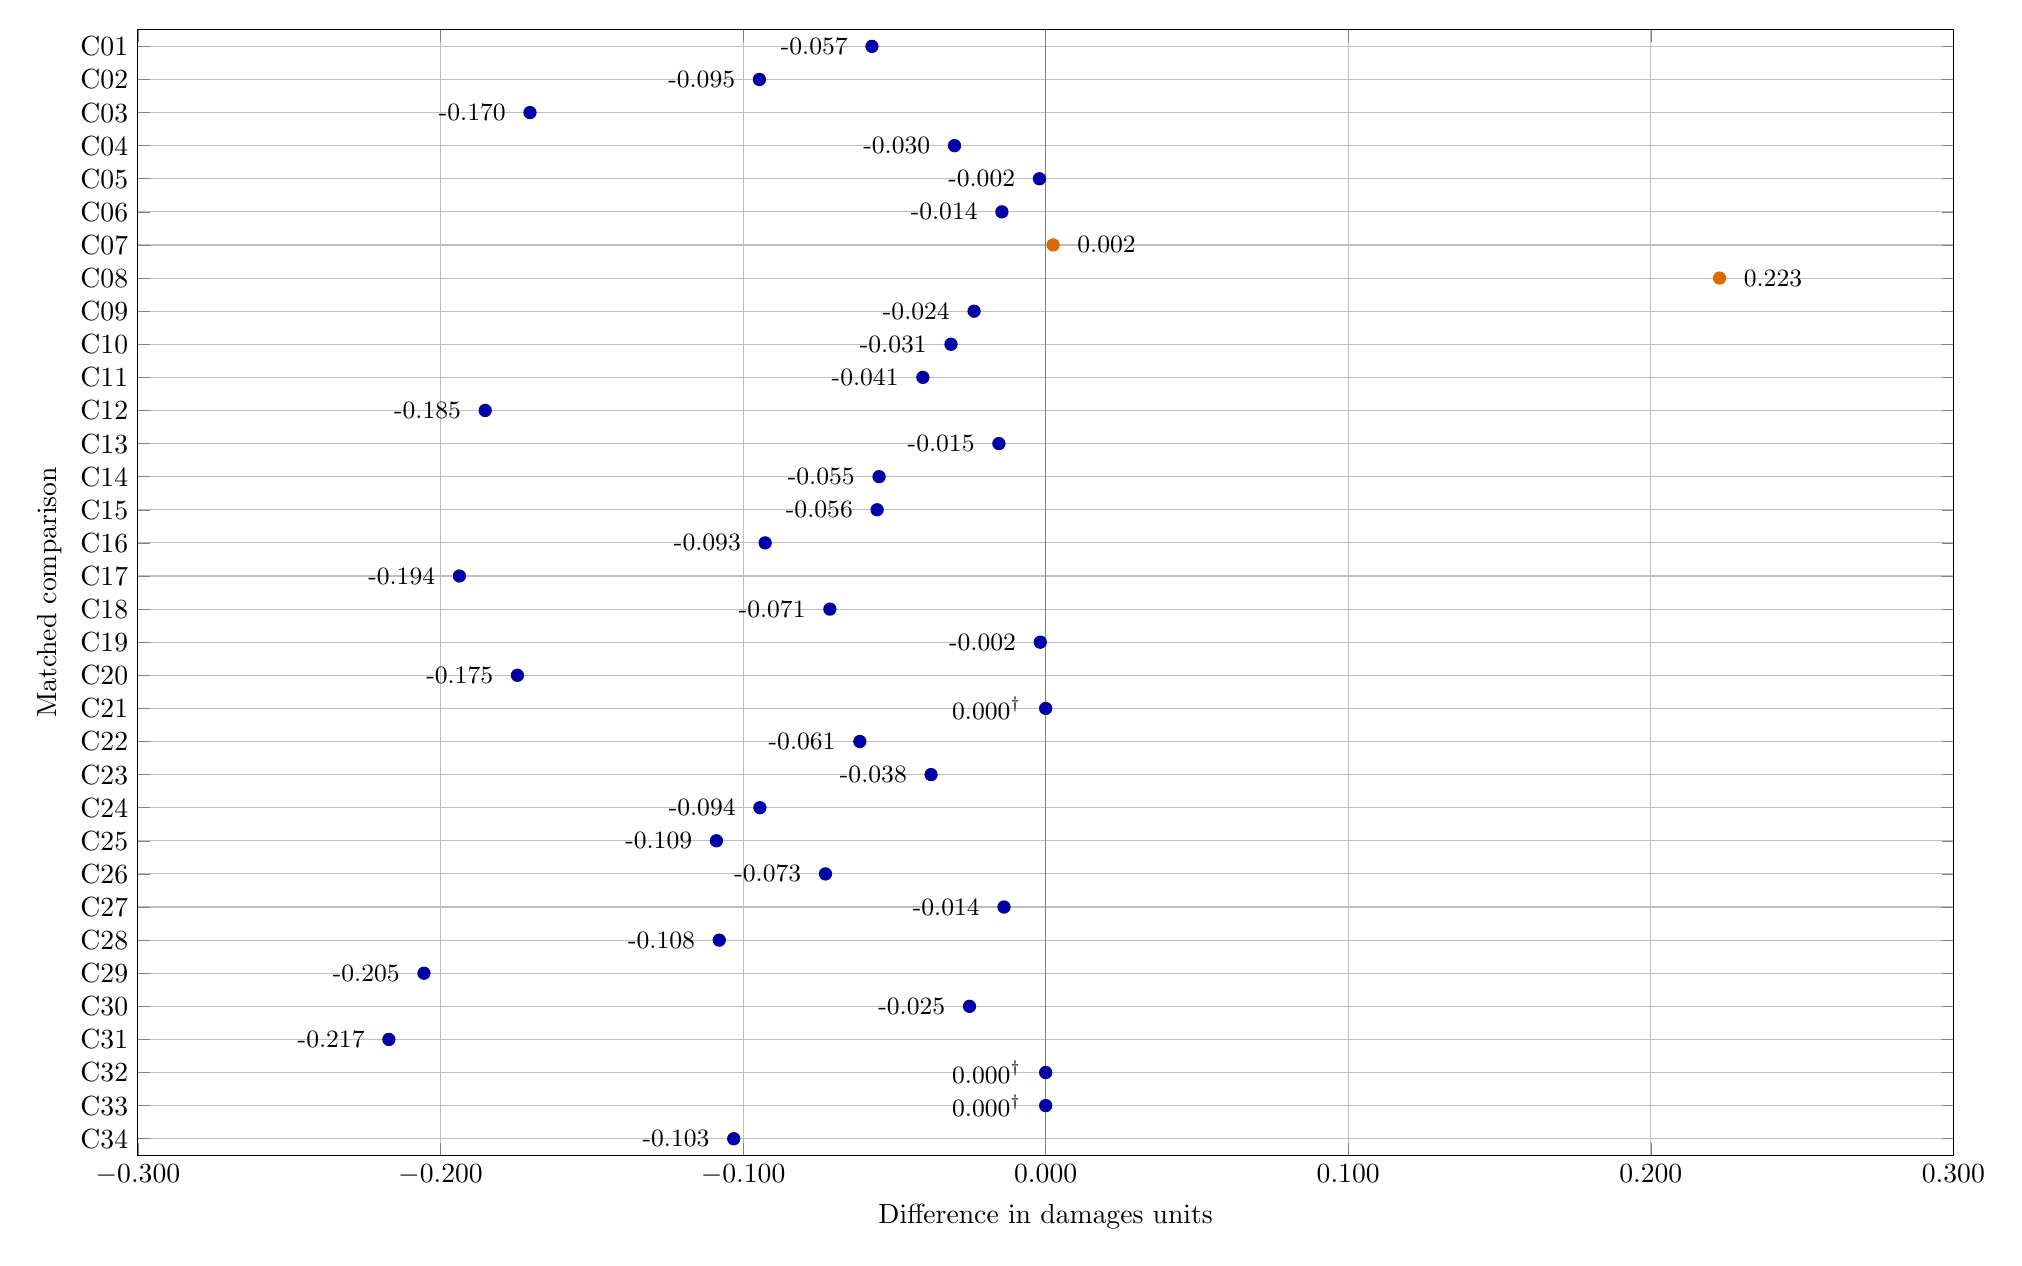
\begin{tikzpicture}\begin{axis}[width=9.7in,height=6.25in,
xmin=-0.30000000000000004,xmax=0.30000000000000004,ymin=.5,ymax=34.5,y dir=reverse,
ytick={1,2,3,4,5,6,7,8,9,10,11,12,13,14,15,16,17,18,19,20,21,22,23,24,25,26,27,28,29,30,31,32,33,34},
yticklabels={C01,C02,C03,C04,C05,C06,C07,C08,C09,C10,C11,C12,C13,C14,C15,C16,C17,C18,C19,C20,C21,C22,C23,C24,C25,C26,C27,C28,C29,C30,C31,C32,C33,C34},
xtick={-0.30000000000000004,-0.20000000000000001,-0.10000000000000001,0,0.10000000000000001,0.20000000000000001,0.30000000000000004},
xticklabel style={/pgf/number format/fixed,/pgf/number format/precision=3,/pgf/number format/fixed zerofill},
xlabel={Difference in damages units},ylabel={Matched comparison},grid=major,clip=false]
\addplot[gray,thin] coordinates {(0,.5) (0,34.5)};
\addplot[only marks,mark=*,mark size=2.2pt,color=blue!65!black] coordinates {(-0.05740706908500004,1)};
\node[font=\small,anchor=east] at (axis cs:-0.062207069085000039,1) {-0.057};
\addplot[only marks,mark=*,mark size=2.2pt,color=blue!65!black] coordinates {(-0.09460005331516852,2)};
\node[font=\small,anchor=east] at (axis cs:-0.099400053315168518,2) {-0.095};
\addplot[only marks,mark=*,mark size=2.2pt,color=blue!65!black] coordinates {(-0.1704307964849997,3)};
\node[font=\small,anchor=east] at (axis cs:-0.1752307964849997,3) {-0.170};
\addplot[only marks,mark=*,mark size=2.2pt,color=blue!65!black] coordinates {(-0.030119513179493018,4)};
\node[font=\small,anchor=east] at (axis cs:-0.034919513179493017,4) {-0.030};
\addplot[only marks,mark=*,mark size=2.2pt,color=blue!65!black] coordinates {(-0.0020538194319791869,5)};
\node[font=\small,anchor=east] at (axis cs:-0.0068538194319791874,5) {-0.002};
\addplot[only marks,mark=*,mark size=2.2pt,color=blue!65!black] coordinates {(-0.014460839805000014,6)};
\node[font=\small,anchor=east] at (axis cs:-0.019260839805000013,6) {-0.014};
\addplot[only marks,mark=*,mark size=2.2pt,color=orange!85!black] coordinates {(0.0024681864885822691,7)};
\node[font=\small,anchor=west] at (axis cs:0.0072681864885822695,7) {0.002};
\addplot[only marks,mark=*,mark size=2.2pt,color=orange!85!black] coordinates {(0.22270808994835478,8)};
\node[font=\small,anchor=west] at (axis cs:0.22750808994835478,8) {0.223};
\addplot[only marks,mark=*,mark size=2.2pt,color=blue!65!black] coordinates {(-0.023663736858750062,9)};
\node[font=\small,anchor=east] at (axis cs:-0.028463736858750061,9) {-0.024};
\addplot[only marks,mark=*,mark size=2.2pt,color=blue!65!black] coordinates {(-0.031288989674999879,10)};
\node[font=\small,anchor=east] at (axis cs:-0.036088989674999877,10) {-0.031};
\addplot[only marks,mark=*,mark size=2.2pt,color=blue!65!black] coordinates {(-0.040575189252830102,11)};
\node[font=\small,anchor=east] at (axis cs:-0.0453751892528301,11) {-0.041};
\addplot[only marks,mark=*,mark size=2.2pt,color=blue!65!black] coordinates {(-0.18522114806384887,12)};
\node[font=\small,anchor=east] at (axis cs:-0.19002114806384887,12) {-0.185};
\addplot[only marks,mark=*,mark size=2.2pt,color=blue!65!black] coordinates {(-0.015456684348179317,13)};
\node[font=\small,anchor=east] at (axis cs:-0.020256684348179316,13) {-0.015};
\addplot[only marks,mark=*,mark size=2.2pt,color=blue!65!black] coordinates {(-0.05506134715704894,14)};
\node[font=\small,anchor=east] at (axis cs:-0.059861347157048939,14) {-0.055};
\addplot[only marks,mark=*,mark size=2.2pt,color=blue!65!black] coordinates {(-0.055705554989999934,15)};
\node[font=\small,anchor=east] at (axis cs:-0.060505554989999932,15) {-0.056};
\addplot[only marks,mark=*,mark size=2.2pt,color=blue!65!black] coordinates {(-0.092712609579850697,16)};
\node[font=\small,anchor=east] at (axis cs:-0.097512609579850695,16) {-0.093};
\addplot[only marks,mark=*,mark size=2.2pt,color=blue!65!black] coordinates {(-0.19375061665499979,17)};
\node[font=\small,anchor=east] at (axis cs:-0.19855061665499979,17) {-0.194};
\addplot[only marks,mark=*,mark size=2.2pt,color=blue!65!black] coordinates {(-0.071308756854931821,18)};
\node[font=\small,anchor=east] at (axis cs:-0.076108756854931819,18) {-0.071};
\addplot[only marks,mark=*,mark size=2.2pt,color=blue!65!black] coordinates {(-0.0017827900981059464,19)};
\node[font=\small,anchor=east] at (axis cs:-0.0065827900981059468,19) {-0.002};
\addplot[only marks,mark=*,mark size=2.2pt,color=blue!65!black] coordinates {(-0.17458552317000081,20)};
\node[font=\small,anchor=east] at (axis cs:-0.17938552317000081,20) {-0.175};
\addplot[only marks,mark=*,mark size=2.2pt,color=blue!65!black] coordinates {(-5.5511151231257827e-17,21)};
\node[font=\small,anchor=east] at (axis cs:-0.004800000000000056,21) {0.000$^{\dagger}$};
\addplot[only marks,mark=*,mark size=2.2pt,color=blue!65!black] coordinates {(-0.0614229244401856,22)};
\node[font=\small,anchor=east] at (axis cs:-0.066222924440185599,22) {-0.061};
\addplot[only marks,mark=*,mark size=2.2pt,color=blue!65!black] coordinates {(-0.037860634858774056,23)};
\node[font=\small,anchor=east] at (axis cs:-0.042660634858774055,23) {-0.038};
\addplot[only marks,mark=*,mark size=2.2pt,color=blue!65!black] coordinates {(-0.094442632889999822,24)};
\node[font=\small,anchor=east] at (axis cs:-0.099242632889999821,24) {-0.094};
\addplot[only marks,mark=*,mark size=2.2pt,color=blue!65!black] coordinates {(-0.10881596850565561,25)};
\node[font=\small,anchor=east] at (axis cs:-0.11361596850565561,25) {-0.109};
\addplot[only marks,mark=*,mark size=2.2pt,color=blue!65!black] coordinates {(-0.072770716049999906,26)};
\node[font=\small,anchor=east] at (axis cs:-0.077570716049999905,26) {-0.073};
\addplot[only marks,mark=*,mark size=2.2pt,color=blue!65!black] coordinates {(-0.013769159764028371,27)};
\node[font=\small,anchor=east] at (axis cs:-0.01856915976402837,27) {-0.014};
\addplot[only marks,mark=*,mark size=2.2pt,color=blue!65!black] coordinates {(-0.10787221141500047,28)};
\node[font=\small,anchor=east] at (axis cs:-0.11267221141500047,28) {-0.108};
\addplot[only marks,mark=*,mark size=2.2pt,color=blue!65!black] coordinates {(-0.20546971243080298,29)};
\node[font=\small,anchor=east] at (axis cs:-0.21026971243080297,29) {-0.205};
\addplot[only marks,mark=*,mark size=2.2pt,color=blue!65!black] coordinates {(-0.025169418329999915,30)};
\node[font=\small,anchor=east] at (axis cs:-0.029969418329999914,30) {-0.025};
\addplot[only marks,mark=*,mark size=2.2pt,color=blue!65!black] coordinates {(-0.21706985414340862,31)};
\node[font=\small,anchor=east] at (axis cs:-0.22186985414340862,31) {-0.217};
\addplot[only marks,mark=*,mark size=2.2pt,color=blue!65!black] coordinates {(-8.3266726846886741e-17,32)};
\node[font=\small,anchor=east] at (axis cs:-0.0048000000000000837,32) {0.000$^{\dagger}$};
\addplot[only marks,mark=*,mark size=2.2pt,color=blue!65!black] coordinates {(-1.1102230246251565e-16,33)};
\node[font=\small,anchor=east] at (axis cs:-0.0048000000000001115,33) {0.000$^{\dagger}$};
\addplot[only marks,mark=*,mark size=2.2pt,color=blue!65!black] coordinates {(-0.10309731209999928,34)};
\node[font=\small,anchor=east] at (axis cs:-0.10789731209999928,34) {-0.103};
\end{axis}\end{tikzpicture}\end{center}
\end{document}